\documentclass[12pt]{article} % use larger type; default would be 10pt

\usepackage[utf8]{inputenc}

%%% PAGE DIMENSIONS
\usepackage{geometry} % to change the page dimensions
\geometry{a4paper} % or letterpaper (US) or a5paper or....
% \geometry{margin=2in} % for example, change the margins to 2 inches all round
% \geometry{landscape} % set up the page for landscape
%   read geometry.pdf for detailed page layout information

\usepackage{graphicx} % support the \includegraphics command and options

% \usepackage[parfill]{parskip} % Activate to begin paragraphs with an empty line rather than an indent

%%% PACKAGES
\usepackage{booktabs} % for much better looking tables
\usepackage{array} % for better arrays (eg matrices) in maths
\usepackage{paralist} % very flexible & customisable lists (eg. enumerate/itemize, etc.)
\usepackage{verbatim} % adds environment for commenting out blocks of text & for better verbatim
\usepackage{listings}
\usepackage{xcolor}
\usepackage{subfig} % make it possible to include more than one captioned figure/table in a single float
% These packages are all incorporated in the memoir class to one degree or another...
% Embedded SQL code style
\definecolor{codegreen}{rgb}{0,0.6,0}
\definecolor{codegray}{rgb}{0.5,0.5,0.5}
\definecolor{codepurple}{rgb}{0.58,0,0.82}
\definecolor{backcolour}{rgb}{0.95,0.95,0.92}

\lstdefinestyle{mystyle}{
    backgroundcolor=\color{backcolour},   
    commentstyle=\color{codegreen},
    keywordstyle=\color{magenta},
    numberstyle=\tiny\color{codegray},
    stringstyle=\color{codepurple},
    basicstyle=\ttfamily\footnotesize,
    breakatwhitespace=false,         
    breaklines=true,                 
    captionpos=b,                    
    keepspaces=true,                 
    numbers=left,                    
    numbersep=5pt,                  
    showspaces=false,                
    showstringspaces=false,
    showtabs=false,                  
    tabsize=2
}

%%% HEADERS & FOOTERS
\usepackage{fancyhdr} % This should be set AFTER setting up the page geometry
\pagestyle{fancy} % options: empty , plain , fancy
\renewcommand{\headrulewidth}{0pt} % customise the layout...
\lhead{}\chead{}\rhead{}
\lfoot{}\cfoot{\thepage}\rfoot{}

%%% SECTION TITLE APPEARANCE
\usepackage{sectsty}
\allsectionsfont{\sffamily\mdseries\upshape} % (See the fntguide.pdf for font help)
% (This matches ConTeXt defaults)

%%% ToC (table of contents) APPEARANCE
\usepackage[nottoc,notlof,notlot]{tocbibind} % Put the bibliography in the ToC
\usepackage[titles,subfigure]{tocloft} % Alter the style of the Table of Contents
\renewcommand{\cftsecfont}{\rmfamily\mdseries\upshape}
\renewcommand{\cftsecpagefont}{\rmfamily\mdseries\upshape} % No bold!

%%% END Article customizations

%%% The "real" document content comes below...

\title{Baze de Date \\ Proiect Inchiriere Apartamente}
\author{Canevschii Daniel}
\date{}

\usepackage{hyperref}
\hypersetup{
    colorlinks,
    citecolor=black,
    filecolor=black,
    linkcolor=black,
    urlcolor=black
}

\begin{document}
\begin{titlepage}
    \centering
    \vspace*{\fill}

    \vspace*{0.5cm}

    \huge\bfseries
    \textit{Baze de Date \\ Proiect Inchiriere Apartamente}

    \vspace*{0.5cm}

    \large Canevschii Daniel

    \vspace*{\fill}
\end{titlepage}

\newpage
\tableofcontents
\newpage
\section{Scopul si obiectivele proiectului}
Scopul proiectului este de a dezvolta o aplicatie care sa faciliteze stocare, extragere si gestionarea informatiei necesare in procesul de detinere sau inchiriere a apartamentelor.
\begin{itemize}
\item Stocarea informatiei despre utilizatorii aplicatiei, cu rolurile corespunzatoare.
\item Stocarea informatiei despre proprietatile detinute de proprietari, precum adresa, numarul de camere, imagini, etc.
\item Inregistrarea contractelor de inchiriere cu datele necesare(stare contract, parti contractate, valabilitate, suma)
\item Pastrarea tuturor tranzactiilor efectuate in cadrul applicatie.
\end{itemize}

\section{Lista cu intrebari ale caror raspunsuri implica interogarea tabelelor} %minim 5
\begin{enumerate}
\item Care sunt apartamentele disponibile spre inchiriere?
\item Care sunt apartamentele (disponibile) din locatia X?
\item Ce apartamente sunt disponibile intre data X - Y?
\item Lista de apartamente cu pret intre X si Y ( mai mare ca X, mai mic ca X)?
\item Lista de proprietati detinute de un anumit proprietar?
\end{enumerate}

\section{Lista cu intrebari ale carori raspunsuri implica adaugarea, actualizarea si stergerea datelor} %minim 10
\begin{enumerate}
\item Cum se adauga un nou user in baza de date?
\item Cum se adauga un nou apartament in baza de date?
\item Cum se depune o cerere de inchiriere a unui apartament?
\item Cum se aproba un contract de inchiriere?
\item Cum se actualizeaza informatie despre un apartament?
\item Cum se modifica informatia unui utilizator?
\item Cum se sterge un utilizator din baza de date?
\item Cum se efectueaza o plata(tranzactie)?
\item Cum se modifica parola unui utilizator?
\item Cum se modifica rolul utilizatorului(proprietar/utilizator)?
\end{enumerate}

\lstset{style=mystyle}

\section{Analiza cererilor de informatii}

\subsection {Care sunt apartamentele disponibile spre inchiriere?}
\begin{enumerate}
\item Se obtine lista apartamentelor ale caror \textit{booking\_id} in \textbf{Booking} e \textit{Ended}.
\end{enumerate}
\lstinputlisting[firstline=1, lastline=5, language=sql]{AnalizaCereri.sql}

\subsection {Care sunt apartamentele (disponibile) din locatia X?}
\begin{enumerate}
\item Se foloseste lista apartamentelor obtinute la punctul anterior, pentru care se verifica daca locatia \textit{X} e aceeasi cu locatia din \textbf{Locations} pentru acelasi \textit{location\_id}.
\end{enumerate}
\lstinputlisting[firstline=7, lastline=16, language=sql]{AnalizaCereri.sql}

\subsection {Ce apartamente sunt disponibile intre data X - Y?}
\subsection {Lista de apartamente cu pret intre X si Y ( mai mare ca X, mai mic ca X)?}
\subsection {Lista de proprietati detinute de un anumit proprietar?}

\section{Modelarea conceptuala(diagrama Entitate - Relatie)}
\subsection {Entitati}
\begin{itemize}
\item Users
\item Properties
\item Locations
\item Bookings
\item Payments
\end{itemize}

\subsection {Legaturi dintre entitati}
\begin{itemize}
\item Users.user\_id [una - multe] Apartments.landlord\_id
\item Users.user\_id [una - multe] Booking.user\_id
\item Users.user\_id [una - multe] Payment.user\_id
\item Apartments.apartment\_id [una - multe] Booking.apartment\_id
\item Booking.booking\_id [una - multe] Payment.booking\_id
\item Locations.location\_id [una - una] Apartments.location\_id
\end{itemize}
\subsection {Determinarea atributelor}

\section{Alegerea SGBD-ului}
Oracle Database

\section{Proiectarea bazei de date (schema logica / schema fizica}
%Tabele(minim3)
%Determinarea coloanelor si tipurilor de date
%Stabilirea legaturilor ditre tabele(definirea cheilor primare si secundare)
%Definirea constrangerilor
%Rafinare
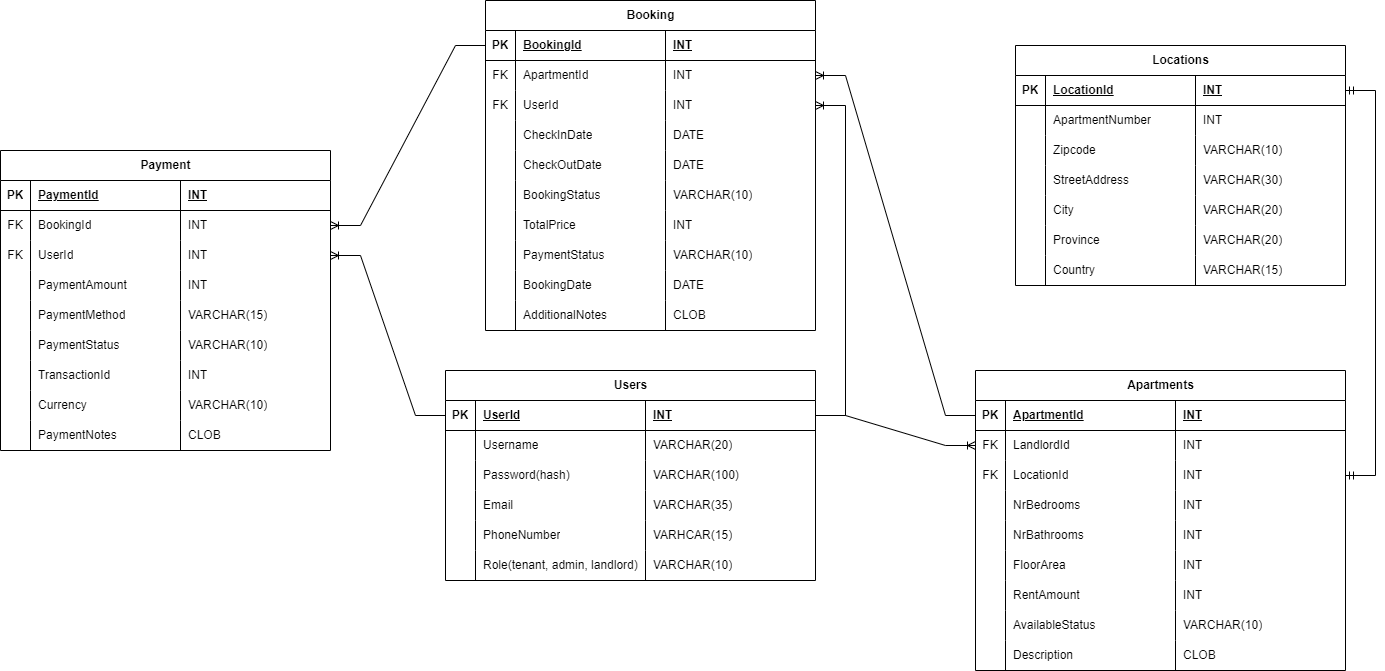
\includegraphics[scale=0.3]{SchemaBD.drawio.png}

\section{Implementarea BD - scripturile SQL (creare, inserare, actualizare, stergere)}
\lstinputlisting[language=sql]{TablesCreate.sql}

\end{document}
